\section{Graph theory}

  \subsection{Definitions}
        
    \subsubsection{Graph}

      A graph $G$ is a pair of sets $(V, E)$ such that $E \subseteq [V]^2$. $V$ or $V(G)$ is a set of arbitrary objects called \emph{vertices} (singular is \emph{vertex}) or \emph{nodes}, while $E$ or $E(G)$ is a set of vertex pairs, called \emph{edges} or \emph{arcs} on occasion; elements of $E$ are two-element subsets of $V$\cite{Diestel2012}.
      
      There are two graph types in respect to edge type: \emph{undirected} and \emph{directed}, pictured on figure \ref{fig:graphs_orientation_undirected} and \ref{fig:graphs_orientation_directed} respectively. In the former, edges are ordered pairs of vertices, i.e. $e = (u, v) = (v, u)$. In the latter they are unordered or just sets of two vertices, that is $e = (u, v) \neq (v, u) = d$.
      \begin{figure}[H]
        \centering        
          \begin{subfigure}[b]{0.25\textwidth}
            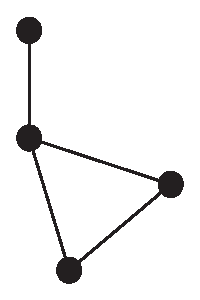
\includegraphics[width=\textwidth]{chapters/02_problem_definition/graph_undirected}
            \caption{An undirected graph.}
            \label{fig:graphs_orientation_undirected}
          \end{subfigure}
          \qquad\qquad\qquad
          \begin{subfigure}[b]{0.25\textwidth}
            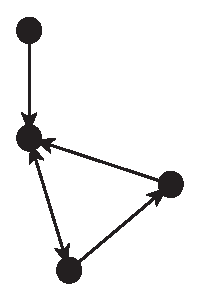
\includegraphics[width=\textwidth]{chapters/02_problem_definition/graph_directed}
            \caption{A directed graph.}
            \label{fig:graphs_orientation_directed}
          \end{subfigure}
        \caption{Types of graphs in respect to orientation.}
        \label{fig:graphs_orientation}
      \end{figure}
      
      Then we have \emph{simple graphs}, where there are no edges from a vertex to itself (called loops) and there are no more than one edge between any two distinct vertices (i.e. edges form sets). On the other side we have \emph{multigraphs} (or \emph{pseudographs}), that may both have loops (not everyone agrees with that) and multiple edges (also called parallel edges) between different vertices (thus they form a multiset).
      \begin{figure}[H]
        \centering        
          \begin{subfigure}[b]{0.25\textwidth}
            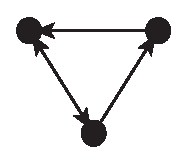
\includegraphics[width=\textwidth]{chapters/02_problem_definition/graph_simple}
            \caption{A simple graph.}
            \label{fig:graphs_orientation_undirected}
          \end{subfigure}
          \qquad\qquad\qquad
          \begin{subfigure}[b]{0.25\textwidth}
            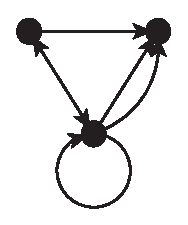
\includegraphics[width=\textwidth]{chapters/02_problem_definition/graph_multi}
            \caption{A multigraph.}
            \label{fig:graphs_orientation_directed}
          \end{subfigure}
        \caption{Types of graphs in respect to edge distinctness.}
        \label{fig:graphs_orientation}
      \end{figure}

      If $(u, v)$ is an edge in an undirected graph then we call $u$ a \emph{neighbour} of $v$ and vice versa. Then we call the number of such neighbours a \emph{degree} of a vertex. In directed graphs however, if $u \rightarrow v$ is a directed edge, then we call $u$ the \emph{predecessor} of $v$, which in turn we call a \emph{successor} of $u$. The \emph{in-degree} of a vertex is the number of predecessors and the \emph{out-degree} of a node is the number of its successors. It is important to note that given $u$ and $v$ and if $u \rightarrow v$ and $v \rightarrow u$ then $u \leftrightarrow v$.

      A graph $H = (U, D)$ is a \emph{subgraph} of $G = (V, E)$ if $U \subseteq V$ and $D \subseteq E$.

    \subsubsection{Paths}

      \paragraph{Path}

        A \emph{path} is a sequence of edges where each successive edge share a vertex and all other edges are disjoint.

      \paragraph{Cycle}

        A \emph{cycle} is a path which starts and ends at the same vertex and has at least one edge.
        
      \begin{figure}[H]
        \centering
        \begin{minipage}[b]{0.43\textwidth}
          \centering
          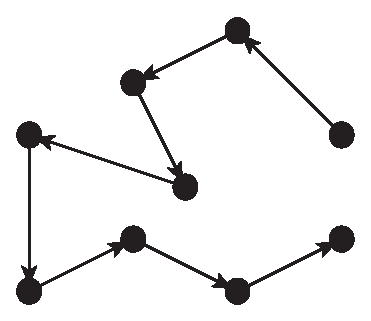
\includegraphics[width=\textwidth]{chapters/02_problem_definition/path}
          \captionof{figure}{A path.}
          \label{fig:path}
        \end{minipage}
        \qquad\qquad
        \begin{minipage}[b]{0.3\textwidth}
          \centering
          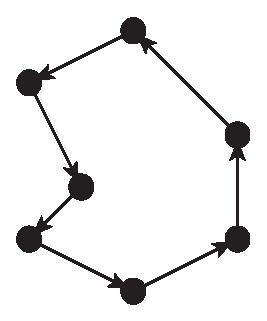
\includegraphics[width=\textwidth]{chapters/02_problem_definition/cycle}
          \captionof{figure}{A cycle.}
          \label{fig:cycle}
        \end{minipage}
      \end{figure}

      \paragraph{Tree}

        A \emph{tree} is a special graph that is a connected acyclic graph. A tree is also a minimal connected graph, meaning that removing any of the edges will make the graph disconnected.

%          http://www.math.uni-hamburg.de/home/diestel/books/graph.theory/preview/Ch1.pdf

      \paragraph{Spanning tree}

        A \emph{spanning tree} of graph $G$ is a subgraph that is a tree and contains all vertices of $G$. Obviously, no spanning trees exist for disconnected graphs.
        
      \begin{figure}[H]
        \centering
        \begin{minipage}[b]{0.35\textwidth}
          \centering
          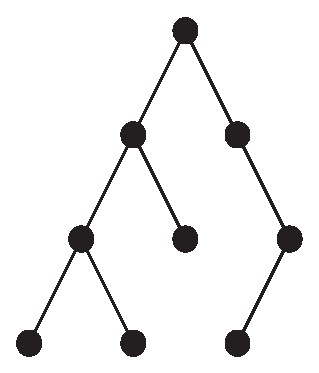
\includegraphics[width=\textwidth]{chapters/02_problem_definition/tree}
          \captionof{figure}{A tree.}
          \label{fig:path}
        \end{minipage}
        \qquad
        \begin{minipage}[b]{0.55\textwidth}
          \centering
          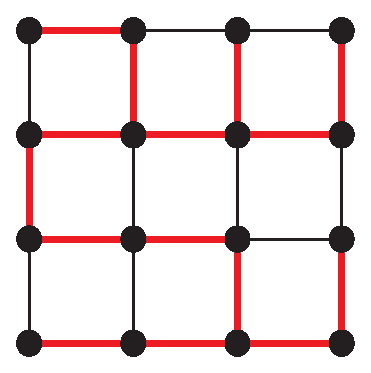
\includegraphics[width=0.7\textwidth]{chapters/02_problem_definition/tree_spanning}
          \captionof{figure}{Spanning tree (bold edges) of grid graph.}
          \label{fig:cycle}
        \end{minipage}
      \end{figure}
    
    \subsubsection{Weighted graph}
    
      A \emph{weighted graph} associates a label (\emph{weight}) with every edge in the graph. Weights are usually real numbers. They may be restricted to rational numbers or integers. The \emph{weight of a path} or the \emph{weight of a tree} in a weighted graph is the sum of the weights of the selected edges. Sometimes a non-edge is labeled by a special weight representing infinity. Sometimes the word \emph{cost} is used instead of weight. When stated without any qualification, a graph is always assumed to be unweighted. In some writing on graph theory the term \emph{network} is a synonym for a weighted graph. A network may be directed or undirected, it may contain special vertices (nodes), such as \emph{source} or \emph{sink}. 
    
    \subsubsection{Graph isomorphism}
        
      An \emph{isomorphism} of a graphs $G$ and $H$ is a bijection between the vertex sets of $G$ and $H$
      \begin{equation}
        f: V(G) \rightarrow V(H)\mbox{,}
      \end{equation}
      such that any two vertices $u$ and $v$ of $G$ are adjacent in $G$ if and only if $f(u)$ and $f(v)$ are adjacent in $H$. This kind of bijection is commonly called \textquote{edge-preserving bijection,} in accordance with the general notion of isomorphism being a structure-preserving bijection.
        
      In the above definition, graphs are understood to be undirected non-labeled non-weighted graphs. However, the notion of isomorphism may be applied to all other variants of the notion of graph, by adding the requirements to preserve the corresponding additional elements of structure: arc directions, edge weights, etc., with the following exception. When spoken about graph labelling with unique labels, commonly taken from the integer range $1,\ldots,n$, where $n$ is the number of the vertices of the graph, two labeled graphs are said to be isomorphic if the corresponding underlying unlabelled graphs are isomorphic.
      
      \begin{table}[H]
        \centering
        \begin{minipage}[b]{0.3\textwidth}
          \centering
          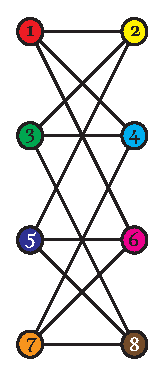
\includegraphics[width=0.55\textwidth]{chapters/02_problem_definition/isomorphism_1}
          \captionof{figure}{Graph $G$.}
        \end{minipage}
        \quad
        \begin{minipage}[b]{0.3\textwidth}
          \centering
          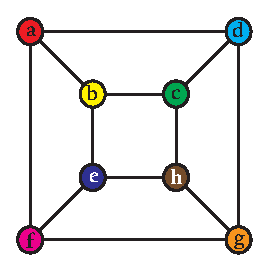
\includegraphics[width=\textwidth]{chapters/02_problem_definition/isomorphism_2}
          \captionof{figure}{Graph $H$.}
        \end{minipage}
        \qquad
        \begin{minipage}[b]{0.3\textwidth}
          \begin{tabularx}{\textwidth}{|C{1}|} \hline
          \rowcolor[gray]{0.75} $f: V(G) \rightarrow V(H)$\\\hline
            $f(1) = a$ \\\hline
            $f(2) = b$ \\\hline
            $f(3) = c$ \\\hline
            $f(4) = d$ \\\hline
            $f(5) = e$ \\\hline
            $f(6) = f$ \\\hline
            $f(7) = g$ \\\hline
            $f(8) = h$ \\\hline
          \end{tabularx}
          \caption{An isomorphism between $G$ and $H$.}
        \end{minipage}
      \end{table}
      
      The notion of \emph{graph isomorphism} allows us to distinguish graph properties inherent to the structures of graphs themselves from properties associated with graph representations: graph drawings, data structures for graphs, graph labelings, etc. For example, if a graph has exactly one cycle, then all graphs in its isomorphism class also have exactly one cycle. On the other hand, in the common case when the vertices of a graph are (represented by) the integers $1, 2, \ldots, N$, then the expression
      \begin{equation}
        \sum_{v \in V(G)} v\cdot\mbox{deg} v\mbox{,}
      \end{equation}
      may be different for two isomorphic graphs.

    \subsubsection{Graph properties}

      In order to focus on the abstract structure of graphs, we define \emph{graph properties} as maintained under all possible \emph{isomorphisms} of a graph. However, there is a distinction referred to this term; specifically, a \emph{property} is usually referred to descriptive characterisations of graphs (i.e. it is a class of graphs), while \emph{invariant} is used for properties expressed quantitatively (i.e. it is a function from graphs to some other set, like $\mathbb{N}$). To avoid naming collisions, from now on I will mention only properties and invariants in the former sense. 

      \paragraph{Graph invariants}

        \subparagraph{Order}

          The \emph{order} of a graph is the number of vertices in a graph and is denoted by $|V(G)|$ or $|G|$.
            
        \subparagraph{Size}

          The \emph{size} of a graph is the number of its edges\cite{Harris2000} in a graph and is denoted by $|E(G)|$ or $||G||$. In an undirected graph, there are $0 \leq E \leq \binom{V}{2}$ and in directed graph: $0 \leq E \leq V(V-1)$. 

        \subparagraph{Eccentricity}    

          The \emph{eccentricity} $\epsilon(v)$ of vertex $v$ is the greatest geodesic distance between $v$ and any other vertex.    
                    
        \subparagraph{Radius}

          The \emph{radius} $r$ of a graph is the minimum eccentricity of any vertex in the graph.

        \subparagraph{Diameter}
        
          The longest of the shortest path lengths is the \emph{diameter} $d$ of a graph. It is the maximum eccentricity of any vertex in the graph. In order to find it, one first need to find the shortest path between each pair of vertices; then the greatest length of any of these paths would be the diameter of the graph.

      \paragraph{Graph properties}

        \subparagraph{Connected}

          Let $G = (V, E)$ be a graph. A non-empty graph $G$ is \emph{connected} if any two of its vertices are linked by a path in $G$, i.e. 
          \begin{equation}
            \forall_{i,j \in \mathbb{N} \cap i,j < |G|} \forall_{v_i \in V} \exists_{v_j \in V} (v_i, v_j) \in E\mbox{.}
          \end{equation}
          In other words, we call a graph \emph{connected} if there is a path from any vertex to any other vertex.

          A maximal connected subgraph of $G$ is a \emph{component} of $G$. The empty graph has no components since connected graphs are non-empty. 

          A graph that is \emph{disconnected} consists of several \emph{connected components}. Two vertices are considered to be in the same conencted component if there is a path between them.

          $G$ is called $k$\emph{-connected} (for $k \in \mathbb{N}$) if $k < |G|$ and $G - X$ is connected for every $X \subseteq V$ with $k > |X|$. Every non-empty graph is 0-connected and 1-connected graphs are precisely non-trivial connected graphs. The greatest integer $k$ such that $G$ is $k$-connected is the \emph{connectivity} $\kappa(G)$ of $G$. Hence graph is disconnected if and only if $\kappa(G) = 0$. The simplest 2-connected graphs are the cycles; all the others can be inductively constructed by adding paths to cycles.

        \subparagraph{Cyclic}
        
          Graph is cyclic when it consists of a single cycle.
          
        \subparagraph{Acyclic}
        
          A graph is called acyclic if there are no subgraphs that are cycles.

        \subparagraph{Bipartite}
        
          In the mathematical field of graph theory, a \emph{bipartite graph} (or \emph{bigraph}) is a graph whose vertices can be divided into two disjoint sets $U$ and $V$ such that every edge connects a vertex in $U$ to one in $V$; that is, $U$ and $V$ are each independent sets. Equivalently, a bipartite graph is a graph that does not contain any odd-length cycles.\cite{Diestel2012,AsratianDenleyHaggkvist}

          The two sets $U$ and $V$ may be thought of as a colouring of the graph with two colours: if one colours all nodes in U blue, and all nodes in V green, each edge has endpoints of differing colours, as is required in the graph colouring problem.\cite{AsratianDenleyHaggkvist,Scheinerman2012} In contrast, such a colouring is impossible in the case of a non-bipartite graph, such as a triangle: after one node is coloured blue and another green, the third vertex of the triangle is connected to vertices of both colours, preventing it from being assigned either colour.
          
          One often writes $G=(U,V,E)$ to denote a bipartite graph whose partition has the parts $U$ and $V$, with $E$ denoting the edges of the graph. If a bipartite graph is not connected, it may have more than one bipartition;\cite{ChartrandZhang2008} in this case, the $(U,V,E)$ notation is helpful in specifying one particular bipartition that may be of importance in an application. If $|U|=|V|$, that is, if the two subsets have equal cardinality, then G is called a balanced bipartite graph.\cite{AsratianDenleyHaggkvist} If vertices on the same side of the bipartition have the same degree, then $G$ is called biregular.
          
          When modelling relations between two different classes of objects, bipartite graphs very often arise naturally. For instance, a graph of football players and clubs, with an edge between a player and a club if the player has played for that club, is a natural example of an affiliation network, a type of bipartite graph used in social network analysis.\cite{WassermanFaust1994}

          Another example where bipartite graphs appear naturally is in the (NP-complete) railway optimisation problem, in which the input is a schedule of trains and their stops, and the goal is to find as small a set of train stations as possible such that every train visits at least one of the chosen stations. This problem can be modelled as a dominating set problem in a bipartite graph that has a vertex for each train and each station and an edge for each pair of a station and a train that stops at that station.\cite{Niedermeier2006}

        \subparagraph{Planar}
        
          In graph theory, a planar graph is a graph that can be embedded in the plane, i.e., it can be drawn on the plane in such a way that its edges intersect only at their endpoints. In other words, it can be drawn in such a way that no edges cross each other.\cite{Trudeau1993,Diestel2012} Such a drawing is called a plane graph or planar embedding of the graph. A plane graph can be defined as a planar graph with a mapping from every node to a point on a plane, and from every edge to a plane curve on that plane, such that the extreme points of each curve are the points mapped from its end nodes, and all curves are disjoint except on their extreme points.

          Every graph that can be drawn on a plane can be drawn on the sphere as well, and vice versa.

          A generalisation of planar graphs are graphs which can be drawn on a surface of a given genus. In this terminology, planar graphs have graph genus $0$, since the plane (and the sphere) are surfaces of genus $0$.

  \subsection{Graphs representation}

    Graphs are usually visualised as an \emph{embeddings}. An embedding of a graph $G(V, E)$ is representation of $G$ on $\Sigma$ plane in which all $v \in V$ are associated to points on $\Sigma$ and each of $e \in E$ are arcs or straight line segments between points corresponding to vertices at both ends of $e$. If no two arcs ever intersect, the embedding of a graph is called \emph{planar}, otherwise it is called a \emph{non-planar}. Because the same graph can have many embeddings that are different, it is important not to confuse the particular embedding with a graph itself. In particular (fig. \ref{fig:graph_planar_nonplanar}), planar graphs can have non-planar embeddings too.

    There are many other ways of graph visualisation, but apart from the above and below, they are not useful for analysis of the data that is a subject of this thesis.

    Graphs can be explicitly represented by either \emph{adjacency matrices} or \emph{adjacency lists}.
        
    The adjacency matrix of a graph $G$ is a $|V| \times |V|$ matrix of indicator variables. Each entry in this matrix indicates whether a particular edge between indexes is or is not in graph $G$:
    \begin{equation}
      A[i, j] = [(i, j) \in E] \mbox{.}
    \end{equation}
    For undirected graph, similar to the edges, the adjacency matrix is always symmetric: $A[i, j] = A[j, i]$. In simple graphs, diagonal entries in $A$ are all zeros since loops are not allowed. The most valuable property of adjacency matrix is that we can decide in $\Theta(1)$ time whether two arbitrary vertices are connected by an edge just by looking at the appropriate elements of the matrix. We also can scan for a list of all vertex neighbours by looking at the corresponding row (or column), which will require $\Theta(V)$ time. The main disadvantage is that this matrix will always take $\Theta(V^2)$ space regardless of how many edges the graph really have. This makes adjacency matrices efficient for \emph{dense} graphs.

    On the other hand, adjacency lists are good when dealing with \emph{sparse} graphs (graphs with relatively small number of edges). Adjacency list is an array of linked lists (one per vertex). For undirected graphs each edge $(u, v)$ is stored twice: once in $u\mbox{'s}$ neighbourhood and once in $v\mbox{'s}$ neighbour list. For directed graph each edge is stored only once. Either way, adjacency list will take $O(V+E)$ space; listing all the neighbours of $v$ vertex takes $O(1+deg(v))$ time (by scanning the neighbour list). We can determine whether $(u, v)$ is an edge by scanning neighbours of $u$ in $O(1+deg(u)$ time.

